%%%% Paramétrage du cours %%%%
\def\xxactivite{Cours}
\def\xxauteur{\textsl{Xavier Pessoles \& Anthony Meurdefroid}}

\fichefalse
\proftrue
\tdfalse
\courstrue

\def\xxnumchapitre{Chapitre 1 \vspace{.2cm}}
\def\xxchapitre{\hspace{.12cm} Introduction}

\def\xxcompetences{%
\textsl{%
\textbf{Savoirs et compétences :}\\
\begin{itemize}[label=\ding{112},font=\color{ocre}] 
\item Analyser les principes d'intelligence artificielle.
\begin{itemize}
\item Régression et classification, apprentissages supervisé et non supervisé.
\item Phases d'apprentissage et d'inférence.
\item Modèle linéaire monovariable ou multivariable.
\item Réseaux de neurones (couches d'entrée, cachées et de sortie, neurones, biais, poids et fonction d'activation).
\end{itemize}
\item Interpréter et vérifier la cohérence des résultats obtenus expérimentalement, analytiquement : Ordre de grandeur. Matrice de confusion (tableau de contingence), sensibilité et spécificité d'un test.
\item Résoudre un problème en utilisant une solution d'intelligence artificielle : 
\begin{itemize}
\item Apprentissage supervisé.
\item Choix des données d'apprentissage. 
\item Mise en œuvre des algorithmes (réseaux de neurones, $k$ plus proches voisins et régression linéaire multiple).
\item Phases d'apprentissage et d'inférence.
\end{itemize}
%\item \textit{Mod2.C17} : torseur dynamique
%\item \textit{Mod2.C17.SF1} : déterminer le torseur dynamique d’un solide, ou d’un ensemble de solides, par rapport à un autre solide
%\item \textit{Mod2.C15} : matrice d'inertie
%\item \textit{Res1.C2} : principe fondamental de la dynamique
%\item \textit{Res1.C1.SF1} : proposer une démarche permettant la détermination de la loi de mouvement
%\item \textit{Res1.C2.SF1} : proposer une méthode permettant la détermination d’une inconnue de liaison
\end{itemize}
}}



\def\xxfigures{
}%figues de la page de garde

\iflivret
\pagestyle{empty}


%%%%%%%% PAGE DE GARDE COURS
\ifcours
% ==== BANDEAU DES TITRES ==== 
\begin{tikzpicture}[remember picture,overlay]
\node at (current page.north west)
{\begin{tikzpicture}[remember picture,overlay]
\node[anchor=north west,inner sep=0pt] at (0,0) {\includegraphics[width=\paperwidth]{\thechapterimage}};
\draw[anchor=west] (-2cm,-8cm) node [line width=2pt,rounded corners=15pt,draw=ocre,fill=white,fill opacity=0.6,inner sep=40pt]{\strut\makebox[22cm]{}};
\draw[anchor=west] (1cm,-8cm) node {\huge\sffamily\bfseries\color{black} %
\begin{minipage}{1cm}
\rotatebox{90}{\LARGE\sffamily\textsc{\color{ocre}\textbf{\xxnumpartie}}}
\end{minipage} \hfill
\begin{minipage}[c]{14cm}
\begin{titrepartie}
\begin{flushright}
\renewcommand{\baselinestretch}{1.1} 
\Large\sffamily\textsc{\textbf{\xxpartie}}
\renewcommand{\baselinestretch}{1} 
\end{flushright}
\end{titrepartie}
\end{minipage} \hfill
\begin{minipage}[c]{3.5cm}
{\large\sffamily\textsc{\textbf{\color{ocre} \discipline}}}
\end{minipage} 
 };
\end{tikzpicture}};
\end{tikzpicture}
% ==== FIN BANDEAU DES TITRES ==== 


% ==== ONGLET 
\begin{tikzpicture}[overlay]
\node[shape=rectangle, 
      rounded corners = .25 cm,
	  draw= ocre,
	  line width=2pt, 
	  fill = ocre!10,
	  minimum width  = 2.5cm,
	  minimum height = 3cm,] at (18.3cm,0) {};
\node at (17.7cm,0) {\rotatebox{90}{\textbf{\Large\color{ocre}{\classe}}}};
%{};
\end{tikzpicture}
% ==== FIN ONGLET 


\vspace{3.5cm}

\begin{tikzpicture}[remember picture,overlay]
\draw[anchor=west] (-2cm,-6cm) node {\huge\sffamily\bfseries\color{black} %
\begin{minipage}{2cm}
\begin{center}
\LARGE\sffamily\textsc{\color{ocre}\textbf{\xxactivite}}
\end{center}
\end{minipage} \hfill
\begin{minipage}[c]{15cm}
\begin{titrechapitre}
\renewcommand{\baselinestretch}{1.1} 
\Large\sffamily\textsc{\textbf{\xxnumchapitre}}

\Large\sffamily\textsc{\textbf{\xxchapitre}}
\vspace{.5cm}

\renewcommand{\baselinestretch}{1} 
\normalsize\normalfont
\xxcompetences
\end{titrechapitre}
\end{minipage}  };
\end{tikzpicture}
\vfill

\begin{flushright}
\begin{minipage}[c]{.3\linewidth}
\begin{center}
\xxfigures
\end{center}
\end{minipage}\hfill
\begin{minipage}[c]{.6\linewidth}
\startcontents
%\printcontents{}{1}{}
\printcontents{}{1}{}
\end{minipage}
\end{flushright}

\begin{tikzpicture}[remember picture,overlay]
\draw[anchor=west] (4.5cm,-.7cm) node {
\begin{minipage}[c]{.2\linewidth}
\begin{flushright}

\includegraphics[width=2cm]{logoCC}
\end{flushright}
\end{minipage}
\begin{minipage}[c]{.2\linewidth}
\textsl{\xxauteur} \\
\textsl{\classe}
\end{minipage}
 };
\end{tikzpicture}

\newpage
\pagestyle{fancy}

%\newpage
%\pagestyle{fancy}

\else
\fi
%% FIN PAGE DE GARDE DES COURS

%%%%%%%% PAGE DE GARDE TD
\iftd

% BANDEAU EXO
\iflivret % SI LIVRET ET TD
\begin{tikzpicture}[remember picture,overlay]
\draw[anchor=west] (-2cm,-3.3cm) node {\huge\sffamily\bfseries\color{black} %
\begin{minipage}{5cm}
\begin{center}
\LARGE\sffamily\color{ocre}\textbf{\textsc{\xxactivite}}

\begin{center}
\xxfigures
\end{center}

\end{center}
\end{minipage} \hfill
\begin{minipage}[c]{12cm}
\begin{titrechapitre}
\renewcommand{\baselinestretch}{1.1} 
\large\sffamily\textbf{\textsc{\xxtitreexo}}

\small\sffamily{\textbf{\textit{\color{black!70}\xxsourceexo}}}
\vspace{.5cm}

\renewcommand{\baselinestretch}{1} 
\normalsize\normalfont
\xxcompetences
\end{titrechapitre}
\end{minipage}};
\end{tikzpicture}
\else % ELSE NOT LIVRET
\begin{tikzpicture}[remember picture,overlay]
\draw[anchor=west] (-2cm,-3.5cm) node {\huge\sffamily\bfseries\color{black} %
\begin{minipage}{5cm}
\begin{center}
\LARGE\sffamily\color{ocre}\textbf{\textsc{\xxactivite}}

\begin{center}
\xxfigures
\end{center}

\end{center}
\end{minipage} \hfill
\begin{minipage}[c]{12cm}
\begin{titrechapitre}
\renewcommand{\baselinestretch}{1.1} 
\large\sffamily\textbf{\textsc{\xxtitreexo}}

\small\sffamily{\textbf{\textit{\color{black!70}\xxsourceexo}}}
\vspace{.5cm}

\renewcommand{\baselinestretch}{1} 
\normalsize\normalfont
\xxcompetences
\end{titrechapitre}
\end{minipage}};
\end{tikzpicture}

\fi

\else   % FIN IF TD
\fi


%%%%%%%% PAGE DE GARDE FICHE
\iffiche
\begin{tikzpicture}[remember picture,overlay]
\node at (current page.north west)
{\begin{tikzpicture}[remember picture,overlay]
\draw[anchor=west] (-2cm,\xxYCartouche) node [line width=2pt,rounded corners=15pt,draw=ocre,fill=white,fill opacity=0.6,inner sep=40pt]{\strut\makebox[22cm]{}};
\draw[anchor=west] (1cm,\xxYCartouche) node {\huge\sffamily\bfseries\color{black} %
\begin{minipage}{1cm}
\rotatebox{90}{\LARGE\sffamily\textsc{\color{ocre}\textbf{\xxnumpartie}}}
\end{minipage} \hfill
\begin{minipage}[c]{14cm}
\begin{titrepartie}
\begin{flushright}
\renewcommand{\baselinestretch}{1.1} 
\large\sffamily\textsc{\textbf{\xxpartie} \\} 

\vspace{.2cm}

\normalsize\sffamily\textsc{\textbf{\xxnumchapitre -- \xxchapitre}}
\renewcommand{\baselinestretch}{1} 
\end{flushright}
\end{titrepartie}
\end{minipage} \hfill
\begin{minipage}[c]{3.5cm}
{\large\sffamily\textsc{\textbf{\color{ocre} \discipline}}}
\end{minipage} 
 };
\end{tikzpicture}};
\end{tikzpicture}

\iflivret % SI LIVRET
\begin{tikzpicture}[overlay]
\node[shape=rectangle, 
      rounded corners = .25 cm,
	  draw= ocre,
	  line width=2pt, 
	  fill = ocre!10,
	  minimum width  = 2.5cm,
	  minimum height = 2.5cm,] at (18.5cm,\xxYongletGarde) {};
\node at (17.9cm,\xxYongletGarde) {\rotatebox{90}{\textsf{\textbf{\large\color{ocre}{\classe}}}}};
%{};
\end{tikzpicture}
\else  % SI PAS LIVRET
\iftd %% SI TD et PAS LIVRET
\begin{tikzpicture}[overlay]
\node[shape=rectangle, 
      rounded corners = .25 cm,
	  draw= ocre,
	  line width=2pt, 
	  fill = ocre!10,
	  minimum width  = 2.5cm,
	  minimum height = 2.5cm,] at (18.6cm,\xxYOnget) {}; %% 0.9 par défaut
\node at (18cm,\xxYOnget) {\rotatebox{90}{\textsf{\textbf{\large\color{ocre}{\classe}}}}};
%{};
\end{tikzpicture}

\else % FIN DU SI TD PAS LIVRET 
\begin{tikzpicture}[overlay]
\node[shape=rectangle, 
      rounded corners = .25 cm,
	  draw= ocre,
	  line width=2pt, 
	  fill = ocre!10,
	  minimum width  = 2.5cm,
%	  minimum height = 2.5cm,] at (18.5cm,1.1cm) {}; % \xxYOnget 0.5
	  minimum height = 2.5cm,] at (18.6cm,.5cm) {};
\node at (18cm,.5cm) {\rotatebox{90}{\textsf{\textbf{\large\color{ocre}{\classe}}}}};
%{};
\end{tikzpicture}
\fi
\fi
\else
\fi



\else
\pagestyle{empty}


%%%%%%%% PAGE DE GARDE COURS
\ifcours
% ==== BANDEAU DES TITRES ==== 
\begin{tikzpicture}[remember picture,overlay]
\node at (current page.north west)
{\begin{tikzpicture}[remember picture,overlay]
\node[anchor=north west,inner sep=0pt] at (0,0) {\includegraphics[width=\paperwidth]{\thechapterimage}};
\draw[anchor=west] (-2cm,-8cm) node [line width=2pt,rounded corners=15pt,draw=ocre,fill=white,fill opacity=0.6,inner sep=40pt]{\strut\makebox[22cm]{}};
\draw[anchor=west] (1cm,-8cm) node {\huge\sffamily\bfseries\color{black} %
\begin{minipage}{1cm}
\rotatebox{90}{\LARGE\sffamily\textsc{\color{ocre}\textbf{\xxnumpartie}}}
\end{minipage} \hfill
\begin{minipage}[c]{14cm}
\begin{titrepartie}
\begin{flushright}
\renewcommand{\baselinestretch}{1.1} 
\Large\sffamily\textsc{\textbf{\xxpartie}}
\renewcommand{\baselinestretch}{1} 
\end{flushright}
\end{titrepartie}
\end{minipage} \hfill
\begin{minipage}[c]{3.5cm}
{\large\sffamily\textsc{\textbf{\color{ocre} \discipline}}}
\end{minipage} 
 };
\end{tikzpicture}};
\end{tikzpicture}
% ==== FIN BANDEAU DES TITRES ==== 


% ==== ONGLET 
\begin{tikzpicture}[overlay]
\node[shape=rectangle, 
      rounded corners = .25 cm,
	  draw= ocre,
	  line width=2pt, 
	  fill = ocre!10,
	  minimum width  = 2.5cm,
	  minimum height = 3cm,] at (18.3cm,0) {};
\node at (17.7cm,0) {\rotatebox{90}{\textbf{\Large\color{ocre}{\classe}}}};
%{};
\end{tikzpicture}
% ==== FIN ONGLET 


\vspace{3.5cm}

\begin{tikzpicture}[remember picture,overlay]
\draw[anchor=west] (-2cm,-6cm) node {\huge\sffamily\bfseries\color{black} %
\begin{minipage}{2cm}
\begin{center}
\LARGE\sffamily\textsc{\color{ocre}\textbf{\xxactivite}}
\end{center}
\end{minipage} \hfill
\begin{minipage}[c]{15cm}
\begin{titrechapitre}
\renewcommand{\baselinestretch}{1.1} 
\Large\sffamily\textsc{\textbf{\xxnumchapitre}}

\Large\sffamily\textsc{\textbf{\xxchapitre}}
\vspace{.5cm}

\renewcommand{\baselinestretch}{1} 
\normalsize\normalfont
\xxcompetences
\end{titrechapitre}
\end{minipage}  };
\end{tikzpicture}
\vfill

\begin{flushright}
\begin{minipage}[c]{.3\linewidth}
\begin{center}
\xxfigures
\end{center}
\end{minipage}\hfill
\begin{minipage}[c]{.6\linewidth}
\startcontents
%\printcontents{}{1}{}
\printcontents{}{1}{}
\end{minipage}
\end{flushright}

\begin{tikzpicture}[remember picture,overlay]
\draw[anchor=west] (4.5cm,-.7cm) node {
\begin{minipage}[c]{.2\linewidth}
\begin{flushright}

\includegraphics[width=2cm]{logoCC}
\end{flushright}
\end{minipage}
\begin{minipage}[c]{.2\linewidth}
\textsl{\xxauteur} \\
\textsl{\classe}
\end{minipage}
 };
\end{tikzpicture}

\newpage
\pagestyle{fancy}

%\newpage
%\pagestyle{fancy}

\else
\fi
%% FIN PAGE DE GARDE DES COURS

%%%%%%%% PAGE DE GARDE TD
\iftd

% BANDEAU EXO
\iflivret % SI LIVRET ET TD
\begin{tikzpicture}[remember picture,overlay]
\draw[anchor=west] (-2cm,-3.3cm) node {\huge\sffamily\bfseries\color{black} %
\begin{minipage}{5cm}
\begin{center}
\LARGE\sffamily\color{ocre}\textbf{\textsc{\xxactivite}}

\begin{center}
\xxfigures
\end{center}

\end{center}
\end{minipage} \hfill
\begin{minipage}[c]{12cm}
\begin{titrechapitre}
\renewcommand{\baselinestretch}{1.1} 
\large\sffamily\textbf{\textsc{\xxtitreexo}}

\small\sffamily{\textbf{\textit{\color{black!70}\xxsourceexo}}}
\vspace{.5cm}

\renewcommand{\baselinestretch}{1} 
\normalsize\normalfont
\xxcompetences
\end{titrechapitre}
\end{minipage}};
\end{tikzpicture}
\else % ELSE NOT LIVRET
\begin{tikzpicture}[remember picture,overlay]
\draw[anchor=west] (-2cm,-3.5cm) node {\huge\sffamily\bfseries\color{black} %
\begin{minipage}{5cm}
\begin{center}
\LARGE\sffamily\color{ocre}\textbf{\textsc{\xxactivite}}

\begin{center}
\xxfigures
\end{center}

\end{center}
\end{minipage} \hfill
\begin{minipage}[c]{12cm}
\begin{titrechapitre}
\renewcommand{\baselinestretch}{1.1} 
\large\sffamily\textbf{\textsc{\xxtitreexo}}

\small\sffamily{\textbf{\textit{\color{black!70}\xxsourceexo}}}
\vspace{.5cm}

\renewcommand{\baselinestretch}{1} 
\normalsize\normalfont
\xxcompetences
\end{titrechapitre}
\end{minipage}};
\end{tikzpicture}

\fi

\else   % FIN IF TD
\fi


%%%%%%%% PAGE DE GARDE FICHE
\iffiche
\begin{tikzpicture}[remember picture,overlay]
\node at (current page.north west)
{\begin{tikzpicture}[remember picture,overlay]
\draw[anchor=west] (-2cm,\xxYCartouche) node [line width=2pt,rounded corners=15pt,draw=ocre,fill=white,fill opacity=0.6,inner sep=40pt]{\strut\makebox[22cm]{}};
\draw[anchor=west] (1cm,\xxYCartouche) node {\huge\sffamily\bfseries\color{black} %
\begin{minipage}{1cm}
\rotatebox{90}{\LARGE\sffamily\textsc{\color{ocre}\textbf{\xxnumpartie}}}
\end{minipage} \hfill
\begin{minipage}[c]{14cm}
\begin{titrepartie}
\begin{flushright}
\renewcommand{\baselinestretch}{1.1} 
\large\sffamily\textsc{\textbf{\xxpartie} \\} 

\vspace{.2cm}

\normalsize\sffamily\textsc{\textbf{\xxnumchapitre -- \xxchapitre}}
\renewcommand{\baselinestretch}{1} 
\end{flushright}
\end{titrepartie}
\end{minipage} \hfill
\begin{minipage}[c]{3.5cm}
{\large\sffamily\textsc{\textbf{\color{ocre} \discipline}}}
\end{minipage} 
 };
\end{tikzpicture}};
\end{tikzpicture}

\iflivret % SI LIVRET
\begin{tikzpicture}[overlay]
\node[shape=rectangle, 
      rounded corners = .25 cm,
	  draw= ocre,
	  line width=2pt, 
	  fill = ocre!10,
	  minimum width  = 2.5cm,
	  minimum height = 2.5cm,] at (18.5cm,\xxYongletGarde) {};
\node at (17.9cm,\xxYongletGarde) {\rotatebox{90}{\textsf{\textbf{\large\color{ocre}{\classe}}}}};
%{};
\end{tikzpicture}
\else  % SI PAS LIVRET
\iftd %% SI TD et PAS LIVRET
\begin{tikzpicture}[overlay]
\node[shape=rectangle, 
      rounded corners = .25 cm,
	  draw= ocre,
	  line width=2pt, 
	  fill = ocre!10,
	  minimum width  = 2.5cm,
	  minimum height = 2.5cm,] at (18.6cm,\xxYOnget) {}; %% 0.9 par défaut
\node at (18cm,\xxYOnget) {\rotatebox{90}{\textsf{\textbf{\large\color{ocre}{\classe}}}}};
%{};
\end{tikzpicture}

\else % FIN DU SI TD PAS LIVRET 
\begin{tikzpicture}[overlay]
\node[shape=rectangle, 
      rounded corners = .25 cm,
	  draw= ocre,
	  line width=2pt, 
	  fill = ocre!10,
	  minimum width  = 2.5cm,
%	  minimum height = 2.5cm,] at (18.5cm,1.1cm) {}; % \xxYOnget 0.5
	  minimum height = 2.5cm,] at (18.6cm,.5cm) {};
\node at (18cm,.5cm) {\rotatebox{90}{\textsf{\textbf{\large\color{ocre}{\classe}}}}};
%{};
\end{tikzpicture}
\fi
\fi
\else
\fi



\fi
\setlength{\columnseprule}{.1pt}

\vspace{2cm}
\pagestyle{fancy}
\thispagestyle{plain}



\section{Le neurone}

\subsection{Bref historique}

\subsection{Modèle de neurone}

\begin{defi}[Neurone (ou perceptron)] ~\\


\begin{minipage}[c]{.55\linewidth}
Prenons la représentation suivante pour un neurone. On note :
\begin{itemize}
\item $x_i$ les données de la couche d'entrée;
\item $w_i$ les poids (poids synaptiques);
\item $b$ le biais;
\item $z_0$ la somme pondérée des entrée;
\item $f$ une fonction d'activation; 
\item $\tilde{y}_0$ : la valeur de sortie du neurone.
\end{itemize}
\end{minipage}
\hfill
\begin{minipage}[c]{.4\linewidth}
\begin{center}
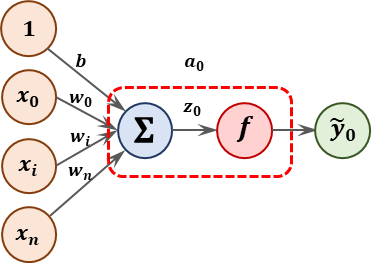
\includegraphics[width=.9\linewidth]{images/fig_01}
\end{center}
\end{minipage}

On a donc, dans un premier temps  :
$$z_0 = b+ \sum\limits_{i=0}^{n} w_i x_i. $$

Après la fonction d'activation, on a donc en sortie du neurone :
$$\tilde{y}_0 = f(z_0)=f \left( b+ \sum\limits_{i=0}^{n} w_i x_i\right).$$

\begin{rem}
\begin{enumerate}
\item La notation tilde ($\tilde{y}_0$) vient du fait que la valeur de sortie d'une neurone est une valeur estimée qu'il faudra comparer à ${y}_0$ valeur de l'étiquette utilisée pour l'apprentissage supervisé.
\item Par la suite, dans la représentation graphique on ne fera pas apparaître la somme pondérée et la fonction d'activation, mais seulement la valeur de sortie du neurone (notée par exemple $a_0$).
\end{enumerate}
\end{rem}

\end{defi}




\begin{defi}[Fonction d'activation]

Les fonctions d'activation sont des fonctions mathématiques appliquées au signal de sortie ($z$). Il est alors possible d'ajouter des non linéarités à la somme pondérée. On donne ci-dessous quelques fonctions usuelles : 

\begin{center}
\begin{tabular}{|c|c|c|c|}
\hline 
Identité & Heaviside & Logistique & Unité de rectification \\
  &  & (sigmoïde) &  linéaire (ReLU) \\
\hline 
&&&\\
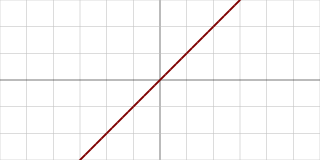
\includegraphics[width=2cm]{images/fig_03_Identite} &
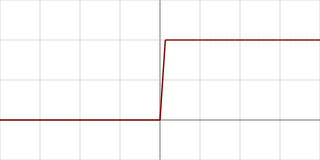
\includegraphics[width=2cm]{images/fig_03_heaviside} &
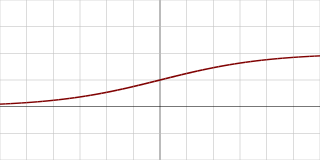
\includegraphics[width=2cm]{images/fig_03_Logistique} &
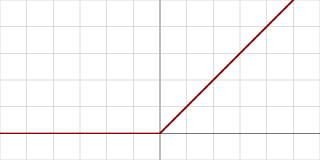
\includegraphics[width=2cm]{images/fig_03_ReLU} \\
&&&\\
$f(x)=x$ & 
$f(x)=\left\{
\begin{array}{l} 
0 \text{ si } x<0 \\ 1 \text{ si } x \geq 0 \\
 \end{array}\right. $
&
$ f(x) = \dfrac{1}{1+\text{e}^{-x}}$ &
$f(x)=\left\{
\begin{array}{l} 
0 \text{ si } x<0 \\ x \text{ si } x \geq 0 \\
 \end{array}\right. $ \\
\hline 
\end{tabular}
\end{center}

\end{defi}


\begin{defi}[Biais]
\end{defi}


\begin{exemple}~\\



\begin{minipage}[c]{.4\linewidth}

Prenons un neurone à deux entrées binaires. 
Initialisation les poids et le biais avec des valeurs aléatoires : $w_0 = -0,3$, $w_1 = 0,8$ et $b=0,2$.

\begin{center}
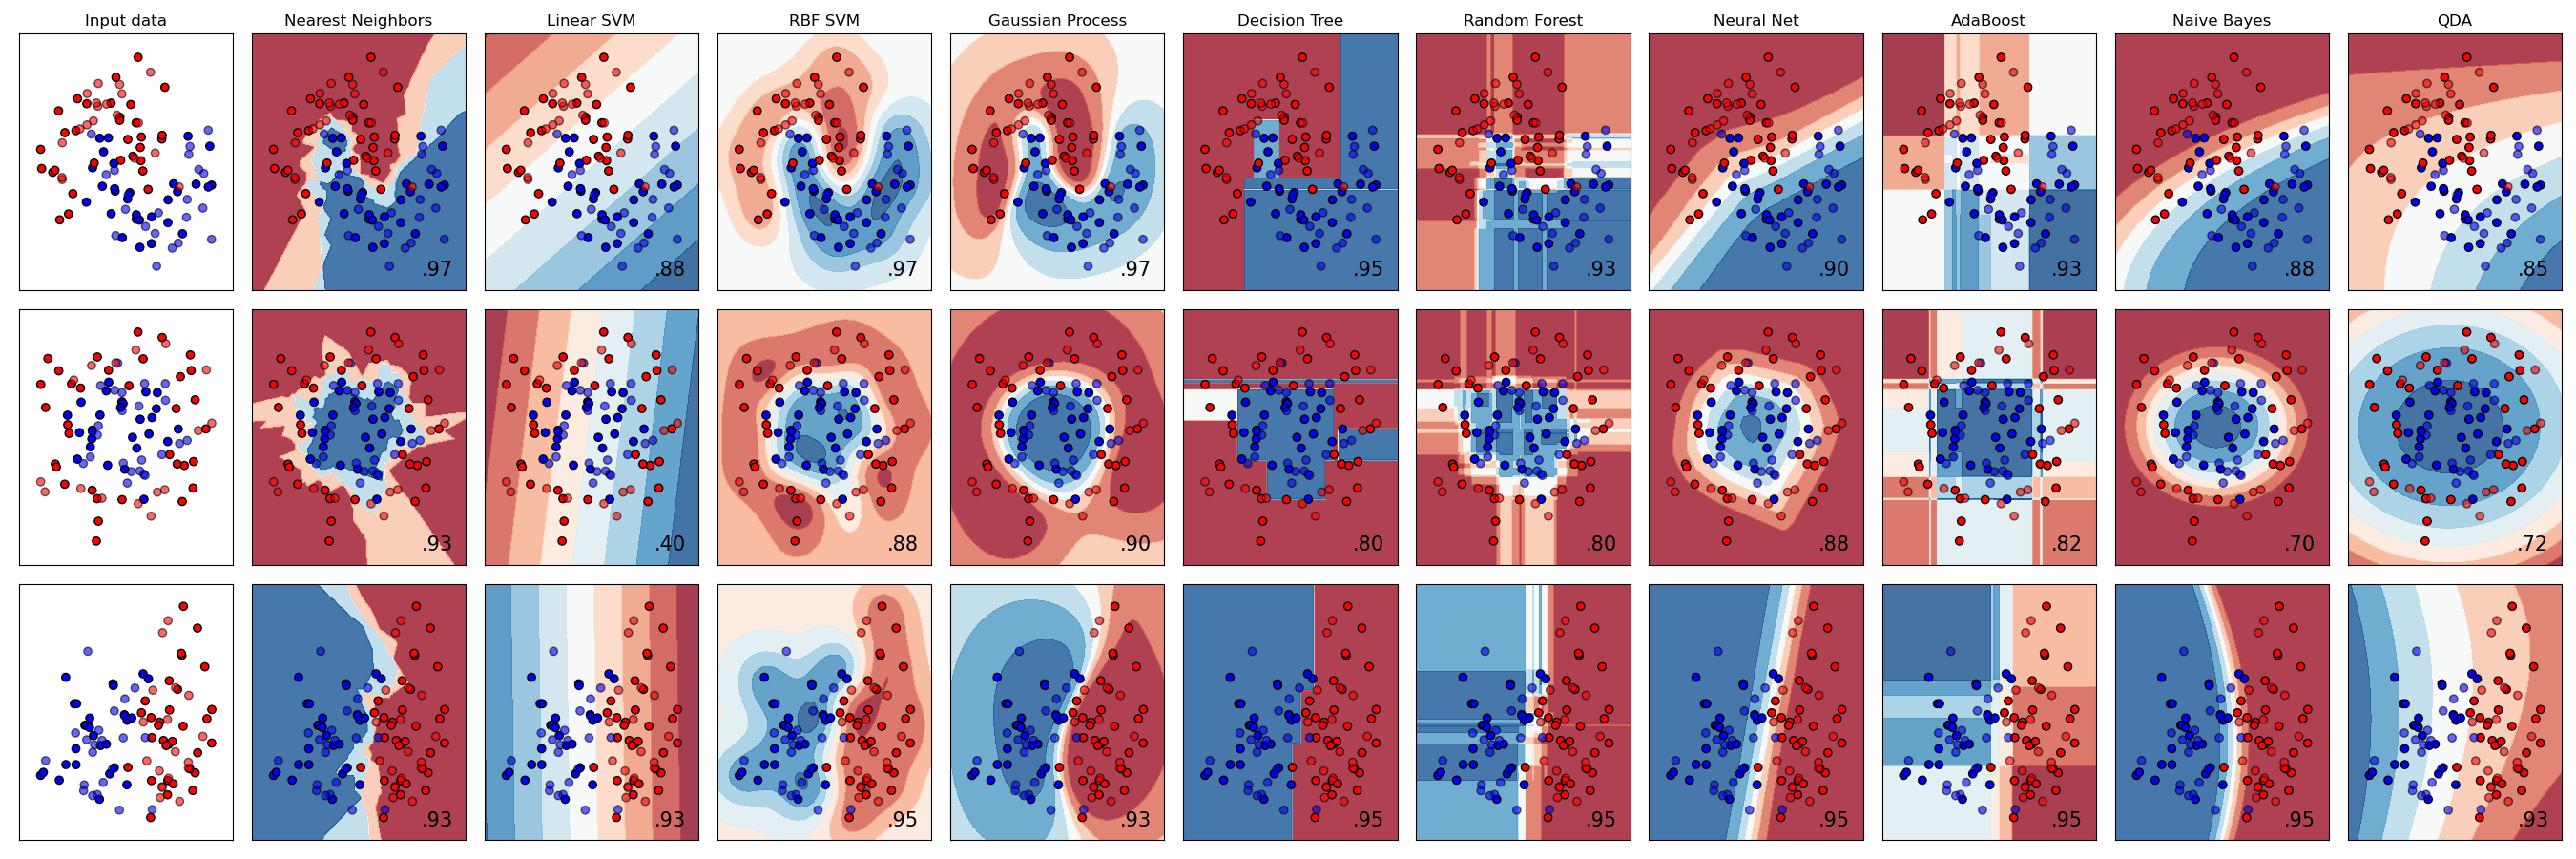
\includegraphics[width=.9\linewidth]{images/fig_02}
\end{center}
\hfill
\end{minipage}
\begin{minipage}[c]{.55\linewidth}


On peut donc évaluer l'ensemble des sorties calculable par le neurone.

\begin{center}
\begin{tabular}{|c|c|| c || c| c|c|c|}
\hline
$x_0$ & $x_1$ & $z$ & Id. & H. & Sig. & ReLu \\
\hline
\hline
0 & 0 & 0,2   &   0,2   &  1 & 0.549 & 0,2 \\
0 & 1 & 1     &    1     &  1 & 0.731  & 1\\
1 & 0 & -0.1  &    -0.1 &  0 &0.475 & 0 \\
1 & 1 & 0.7  &     0.7  &  1 &0.668 & 0.7\\
\hline
\end{tabular}
\end{center}
\end{minipage}

\end{exemple}


\section{Réseaux de neurones}
\url{https://playground.tensorflow.org/}
%LSTM


\subsection{Modélisation d'un réseau de neurones} 

\begin{defi}[Couches] ~\\

Un réseau de neurones va être un ensemble de neurones reliés, par couches, entre eux. 

Dans un réseau de neurones \textbf{dense} tous les neurones de la couche $i$ seront reliés à tous les neurones de la couche $i+1$.

\begin{itemize}
\item Couche d'entrée : cette couche est une copie de l'ensemble des données d'entrées. Le nombre de neurones de cette couche correspond donc aux nombre de données d'entrées.
\item Couche cachée (ou couche intermédiaire) : il s'agit d'une couche qui a une utilité intrinsèque au réseau de neurones. Ajouter des neurone dans cette couche (ou ces couches) permet donc d'ajouter de nouveaux paramètres.  Pour une couche, la même fonction d'activation est utilisée pour tous les neurones. En revanche la fonction d'activation utilisée peut être différente pour deux couches différentes. Les fonctions d'activations des couches intermédiaires sont souvent non linéaires.
\item Couche de sortie : le nombre de neurones de cette couche correspond au nombre de sorties attendues. La fonction d'activation de la couche de sortie est souvent linéaire.
\end{itemize}
%\begin{minipage}[c]{.5\linewidth}
\begin{center}
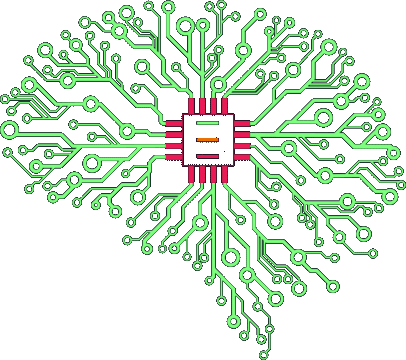
\includegraphics[width=.8\linewidth]{images/fig_04}
\end{center}
%\end{minipage}

Notations : 
\begin{itemize}
\item on note $w^{[l]}_{jk}$ les poids permettant d'aller vers la couche $l$ depuis le neurone $k$ vers le neurone $j$;
\item $b^{[l]}_{j}$ le biais permettant d'aller sur le neurone $j$ de la couche $l$.
\end{itemize}
\end{defi}


\begin{defi}[Paramètres]

Les paramètres du réseau de neurones sont les poids et les biais, autant de valeurs que l’entraînement devra déterminer.

\end{defi}
\begin{methode}[Calcul du nombre de paramètres -- à vérifier]

Soit un jeu de données étiquetées avec $n$ entrées et $p$ sorties.

On construit un réseau possédant $\ell$ couches cachées et $a_\ell$ le nombre de neurones de la couche  $\ell$.

\textbf{Nombre de poids :} $n_w = ...$.

\textbf{Nombre de bais :} $n_b = \sum\limits_{i=1}^{\ell}\left( a_i  \right)+ p$.




\end{methode}
\begin{obj}
Soit un jeu de données étiquetées avec $n$ entrées et $p$ sorties. .


L'objectif de l'apprentissage d'un réseau de neurones est de déterminer l'ensemble des poids et des biais de telle sorte que, 
\end{obj}



\begin{defi}[Hyper paramètres]

Nombre de couvhes
\end{defi}


\subsection{Propagation}

\subsection{Rétropropagation}


\begin{defi}[Quantification de l'erreur]
\end{defi}


\section{Algorithmes d'apprentissage}




\newpage

\section{Définitions}

\begin{itemize}
\item Data scientist
\item machine learning
\item deep learning
\item réseaux de neurons
\item régression
\item data mining
\item bigdata
\item données continues, données discrètes, données nominales, données ordinales, données (semi-)structurées et non structurées

\end{itemize}


\begin{itemize}
\item algorithmes supervisés, non supervisés
\item algorithmes de régression et de classification
\end{itemize}

\begin{defi}[Machine Learning -- Apprentissage automatique -- Wikipedia] 
Champ d'étude de l'intelligence artificielle qui se fonde sur des approches mathématiques et statistiques pour donner aux ordinateurs la capacité d' « apprendre » à partir de données, c'est-à-dire d'améliorer leurs performances à résoudre des tâches sans être explicitement programmés pour chacune. 

La première phase de l'apprentissage consiste à estimer un modèle à partir de données, appelées observations, qui sont disponibles et en nombre fini, lors de la phase de conception du système.

 La seconde phase correspond à la mise en production : le modèle étant déterminé, de nouvelles données peuvent alors être soumises afin d'obtenir le résultat correspondant à la tâche souhaitée.
\end{defi}


\begin{defi}[Apprentissage supervisé -- Apprentissage non supervisé -- Apprentissage par renforcement -- Wikipedia] 
Si les données sont étiquetées (c'est-à-dire que la réponse à la tâche est connue pour ces données), il s'agit d'un apprentissage supervisé. On parle de :
\begin{itemize}
\item classification ou de classement si les étiquettes sont discrètes;
\item régression si elles sont continues.
\end{itemize}

Si le modèle est appris de manière incrémentale en fonction d'une récompense reçue par le programme pour chacune des actions entreprises, on parle d'apprentissage par renforcement. 

Dans le cas le plus général, sans étiquette, on cherche à déterminer la structure sous-jacente des données (qui peuvent être une densité de probabilité) et il s'agit alors d'apprentissage non supervisé.



\end{defi}



\subsection{Quelques définitions}
\begin{defi}{Intelligence Artificielle, première approche}

\end{defi}

\subsection{Le nerf de la guerre, les données}



\subsection{Méthode de résolution de problèmes d'apprentissage supervisé}

\begin{enumerate}
\item Choix des données.
\item Normalisation des données. 
\item Séparation des données ? (entraînement, test, validation)
\item Choix de la méthode d’entraînement (choix d'un modèle, en fonction du type de données, choix des paramètres du modèle)
\item Entraînement du modèle
\item Test du modèle
\item Observation des métriques et visualisation des résultats
\end{enumerate}

\section{Méthode de résolution d'un }

\newpage


1 cours Sur les réseau de neurones

\section{TP : Synthèse d'un contrôleur piloté par réseau de neurones}

TP identification de la boucle ouverte  
\begin{itemize}
\item Comparaison modèle (a)causal / réel
\item Comparaison modèle ANN / réel
\end{itemize}


TP Synthèse du contrôleur PID 
à partir du modèle
To do XP

TP synthèse du contrôleur et implémentation sur une cible. 
Déploiement sur control X ?



\newpage


\newpage

Exemples : 
\url{https://makina-corpus.com/blog/metier/2017/initiation-au-machine-learning-avec-python-pratique}

\begin{thebibliography}{2}
   \bibitem[1]{ref1} Éric Biernat et Michel Lutz. {\it Data science : fondamentaux et études de cas.} Eyrolles.
\end{thebibliography}

